

%\begin{center}
%\end{center}
\begin{flushleft}

\chapter{Set up Process on Visual Studio}

\section{\textbf{Introduction}}
\medskip

Visual Studio Express products provide a free development environment to develop applications for the latest platforms. Visual Studio Express can be downloaded from

\medskip

\url{http://www.visualstudio.com/en-us/products/visual-studio-express-vs.aspx}.

\medskip
The experiments on kinect discussed in this manual are designed using C\# and Windows Presentation Foundation (WPF). Before commencing the discussion of experiments and their code, it is essential to understand how to set up the environment to design the same. This includes adding references, the procedure for which is discussed in this chapter.
This is a prerequisite to the experimenting stage to follow.

\medskip
\textbf{Note : }
At the time of making of this manual, the latest version was Visual Studio Express 2013. The same was used for experimenting with kinect.

\medskip
\subsection{\textbf{ System Requirements}}
\medskip
\textbf{Supported Operating System}

Windows 7 SP1 (x86 and x64), Windows 8 (x86 and x64), Windows 8.1 (x86 and x64), Windows Server 2008 R2 SP1 (x64), Windows Server 2012 (x64) and Windows Server 2012 R2 (x64).

\medskip
\begin{itemize}
\item Hardware Requirements
\medskip
\begin{itemize}
\item 1.6 GHz or faster processor
\item 1 GB of RAM (1.5 GB if running on a virtual machine)
\item 5 GB of available hard disk space
\item 5400 RPM hard drive
\item DirectX 9-capable video card running at 1024 x 768 or higher display resolution
\end{itemize}
\medskip

\medskip
\end{itemize}
\subsection{\textbf{ Set up Procedure}}
\addcontentsline{lof}{figure}{\textbf{Set up procedure on Visual Studio 2013}}

\textbf{Step 1 :}
\medskip

Double click the \textbf{VS Express 2013 for desktop} icon to start the application.
Alternately, one can start the application from start menu as well.
Shown in Figure \ref{fig:e1}.
\medskip

\textbf{Step 2 :}

\medskip
Click on \textbf{New Project} to create a new project.
Shown in Figure \ref{fig:e2}.

\medskip

\textbf{Step 3 :}

\medskip
Select 
\textbf{Visual C\# $\rightarrow$ WPF Application}
Give a project name and save it in the appropriate directory of your choice. In this example the project name is \textbf{my\_expt} saved in the \textbf{experiment} folder.
Shown in Figure \ref{fig:e3}.

\medskip

\textbf{Step 4 :}

\medskip

The project window will open. On the right hand side you will find the \textbf{Solution Explorer}.
Right click on \textbf{my\_expt $\rightarrow$ Add $\rightarrow$ Reference}
Shown in Figure \ref{fig:e4}.

\medskip

\textbf{Step 5 :}

\medskip

The Reference Manager will open. Go to \textbf{Assemblies $\rightarrow$ Extensions} and select \textbf{Microsoft.Kinect}. Click 'OK' to add.
Shown in Figure \ref{fig:e5}.
 
\medskip

\textbf{Step 6 :}

\medskip

In the solution explorer right click on \textbf{Solution 'my\_expt'(1 project) $\rightarrow$ Add $\rightarrow$ Existing Project}
Shown in Figure \ref{fig:e6}.

\medskip

\textbf{Step 7 :}

\medskip

Navigate to \textbf{KinectWpfViewers} folder (provided with this manual) and select \textbf{Microsoft.Samples.Kinect.WpfViewers.csproj}. Click 'Open' to add this project.
Shown in Figure \ref{fig:e7}.

\medskip

\textbf{Step 8 :}

\medskip
Now we need to reference this project.
Right click on \textbf{my\_expt $\rightarrow$ Add $\rightarrow$ Reference}.
Go to \textbf{Solution $\rightarrow$ Projects} and select \textbf{Microsoft.Samples.kinect.WpfViewers}
Shown in Figure \ref{fig:e8}.


\medskip

\textbf{Step 9 :}

\medskip
Now add the final 2 references.
Right click on \textbf{my\_expt $\rightarrow$ Add $\rightarrow$ Reference}.
Go to Browse and navigate to 
\textbf{KinectWpfViewers} folder (provided with this manual) \textbf{$\rightarrow$ bin $\rightarrow$ Debug}
and select the 2 files :
\textbf{Microsoft.Kinect.Toolkit.dll} and
\textbf{Microsoft.Samples.Kinect.WpfViewers.dll}
Click 'OK' to add the same.

Shown in Figure \ref{fig:e9}.
\medskip

\textbf{Step 10 :}

\medskip
This completes the set up process. The Project window after completion of setup is shown in Figure \ref{fig:e10}.
You can now start programming on C\# and WPF for kinect applications

\medskip

\begin{figure}
\begin{center}
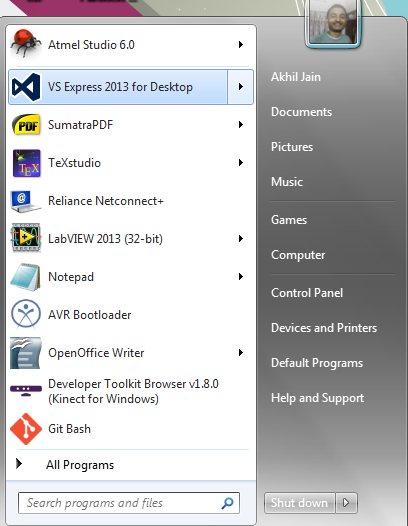
\includegraphics[scale=0.6]{s1}
\end{center}
\caption{Step 1 - Open VS Express 2013 for windows desktop}
\label{fig:e1}
\end{figure}

\medskip
\begin{figure}
\begin{center}
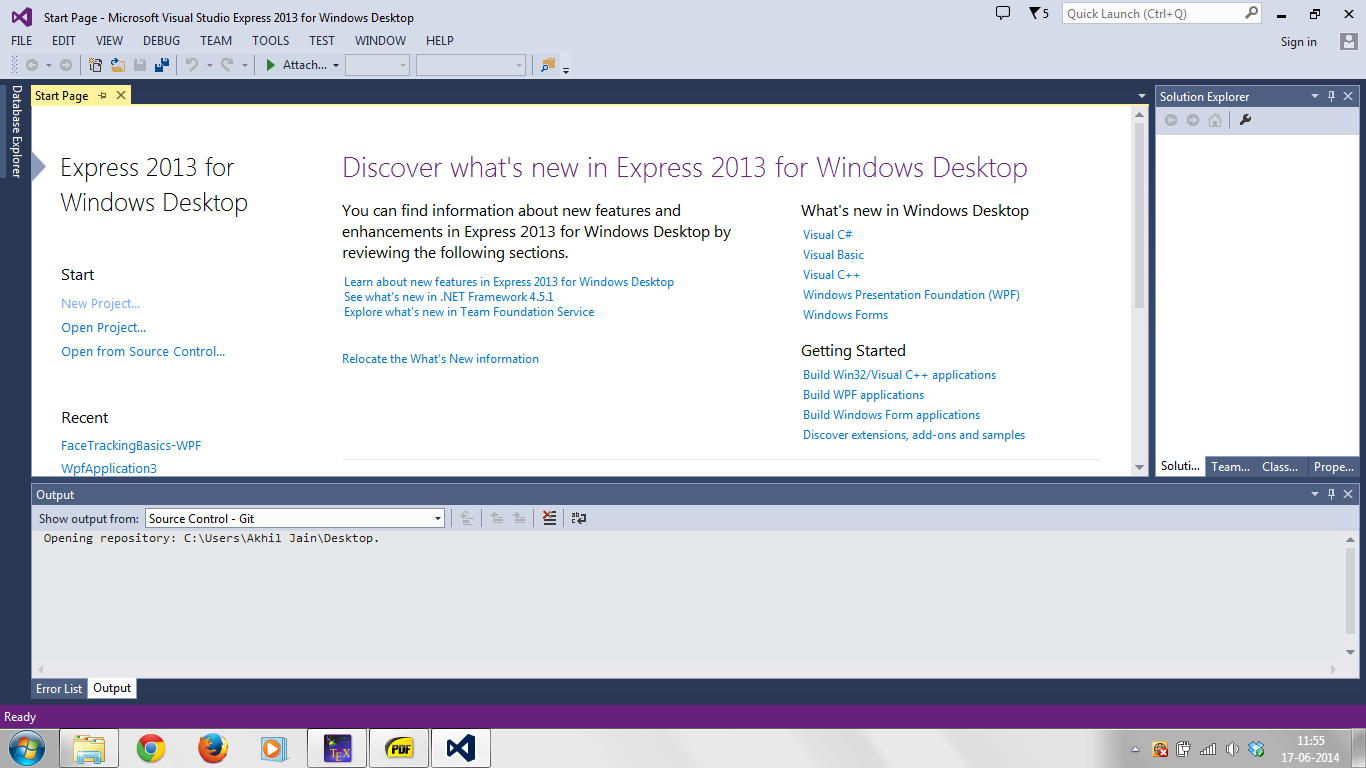
\includegraphics[scale=0.5]{s2}
\end{center}
\caption{Step 2 - Click on New Project}
\label{fig:e2}
\end{figure}
\medskip

\begin{figure}
\begin{center}
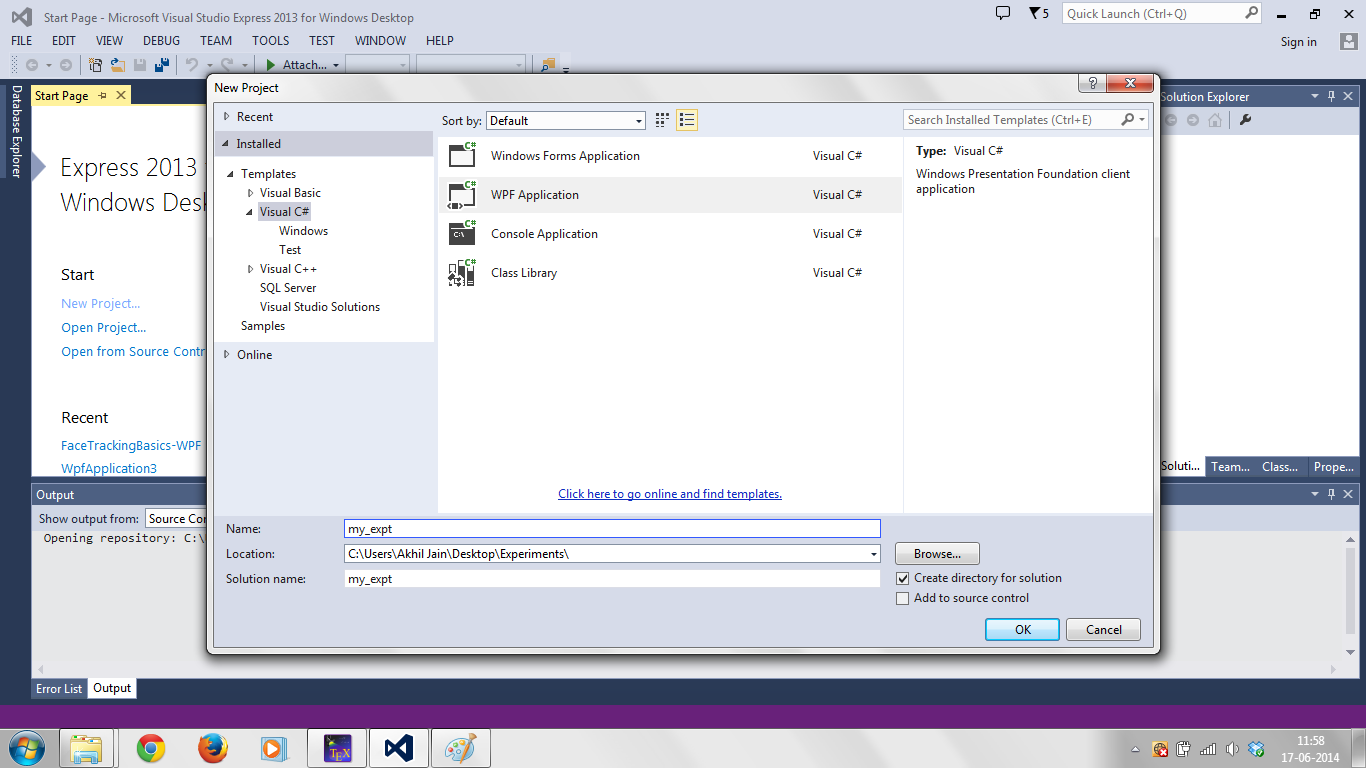
\includegraphics[scale=0.5]{s3}
\end{center}
\caption{Step 3 - Create a new C\# project}
\label{fig:e3}
\end{figure}

\medskip
\begin{figure}
\begin{center}
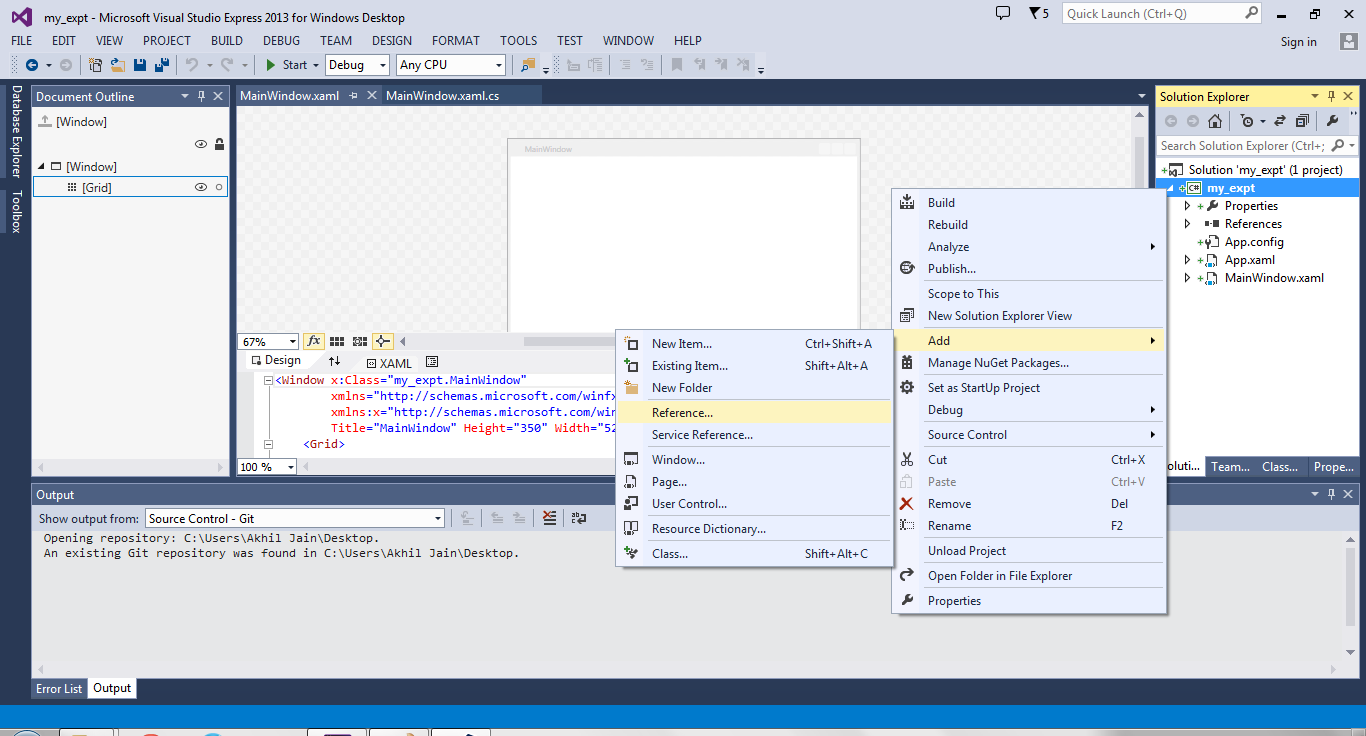
\includegraphics[scale=0.5]{s4}
\end{center}
\caption{Step 4 - Adding Reference}
\label{fig:e4}
\end{figure}

\medskip
\begin{figure}
\begin{center}
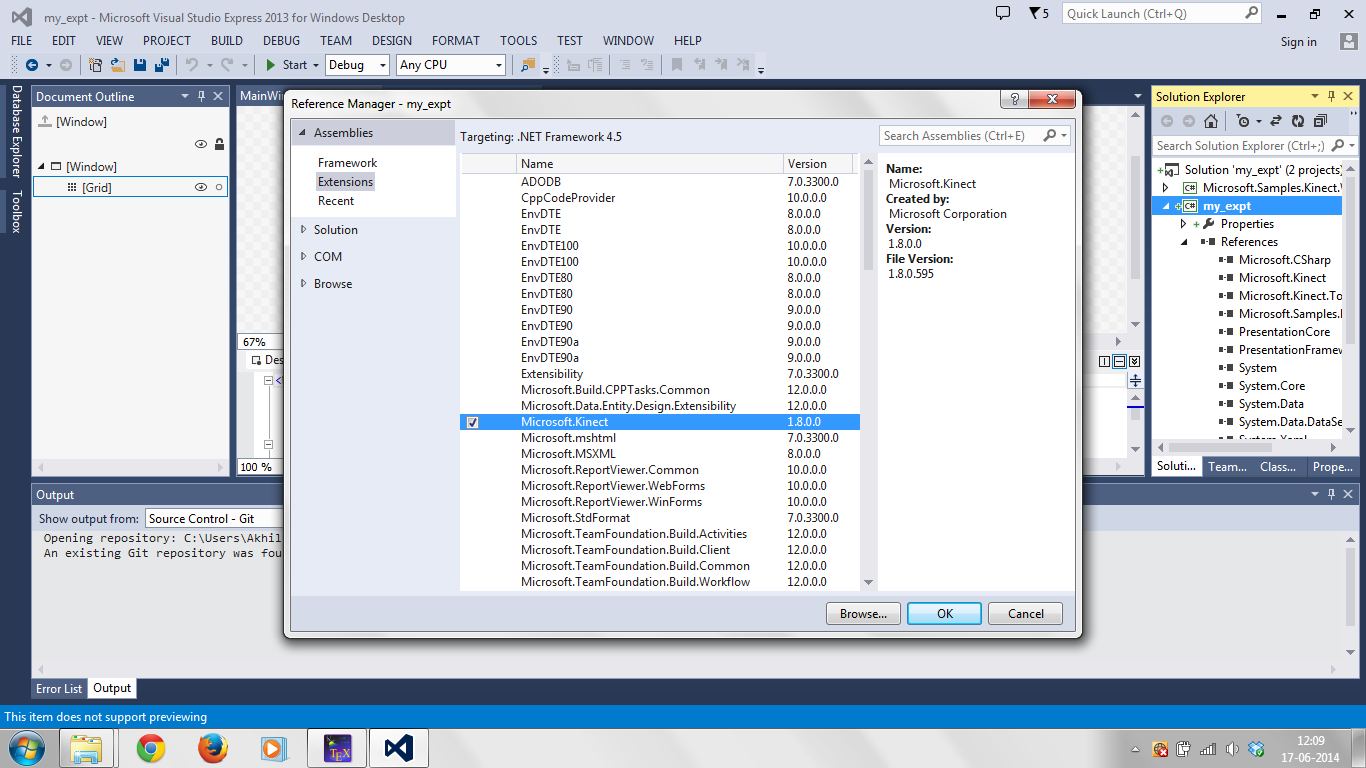
\includegraphics[scale=0.5]{s5}
\end{center}
\caption{Step 5 - Add reference to Microsoft.Kinect}
\label{fig:e5}
\end{figure}

\medskip
\begin{figure}
\begin{center}
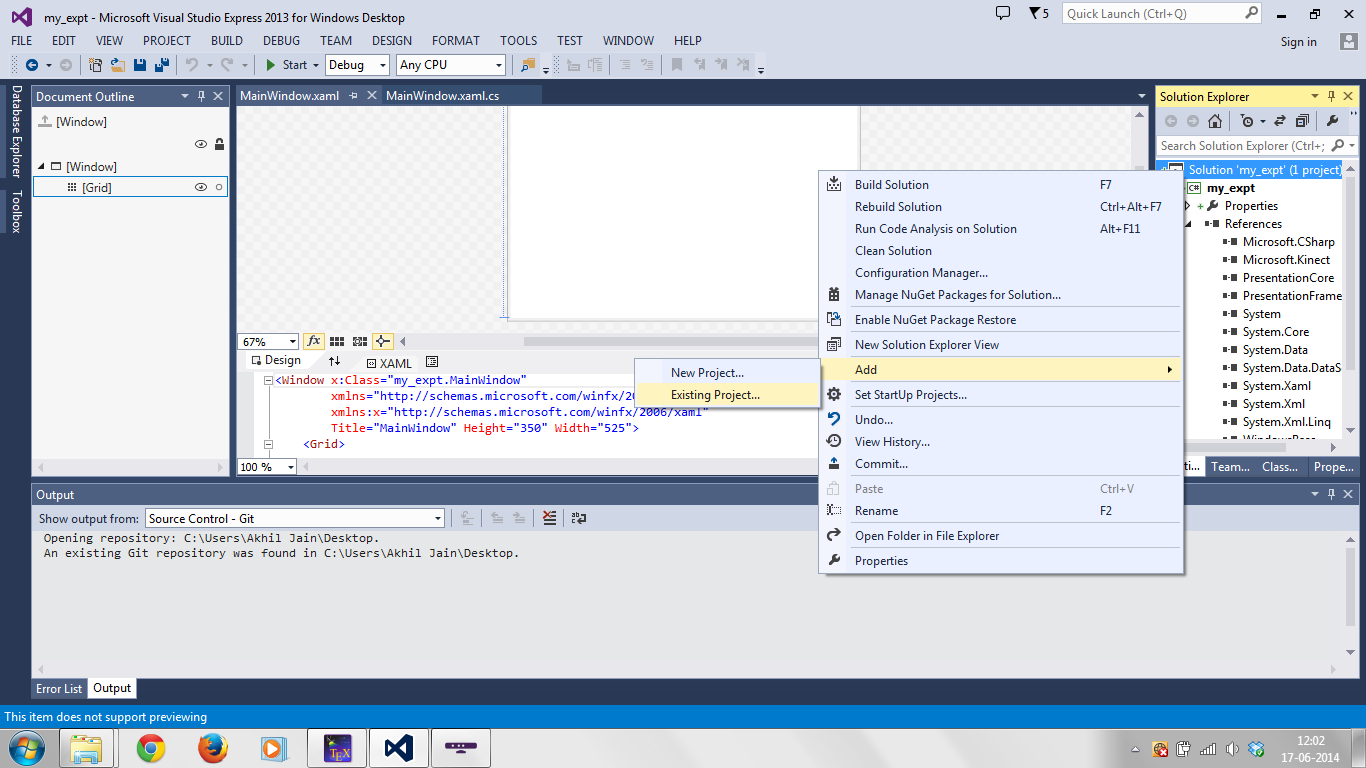
\includegraphics[scale=0.5]{s6}
\end{center}
\caption{Step 6 - Adding existing project}
\label{fig:e6}
\end{figure}
\medskip
\begin{figure}
\begin{center}
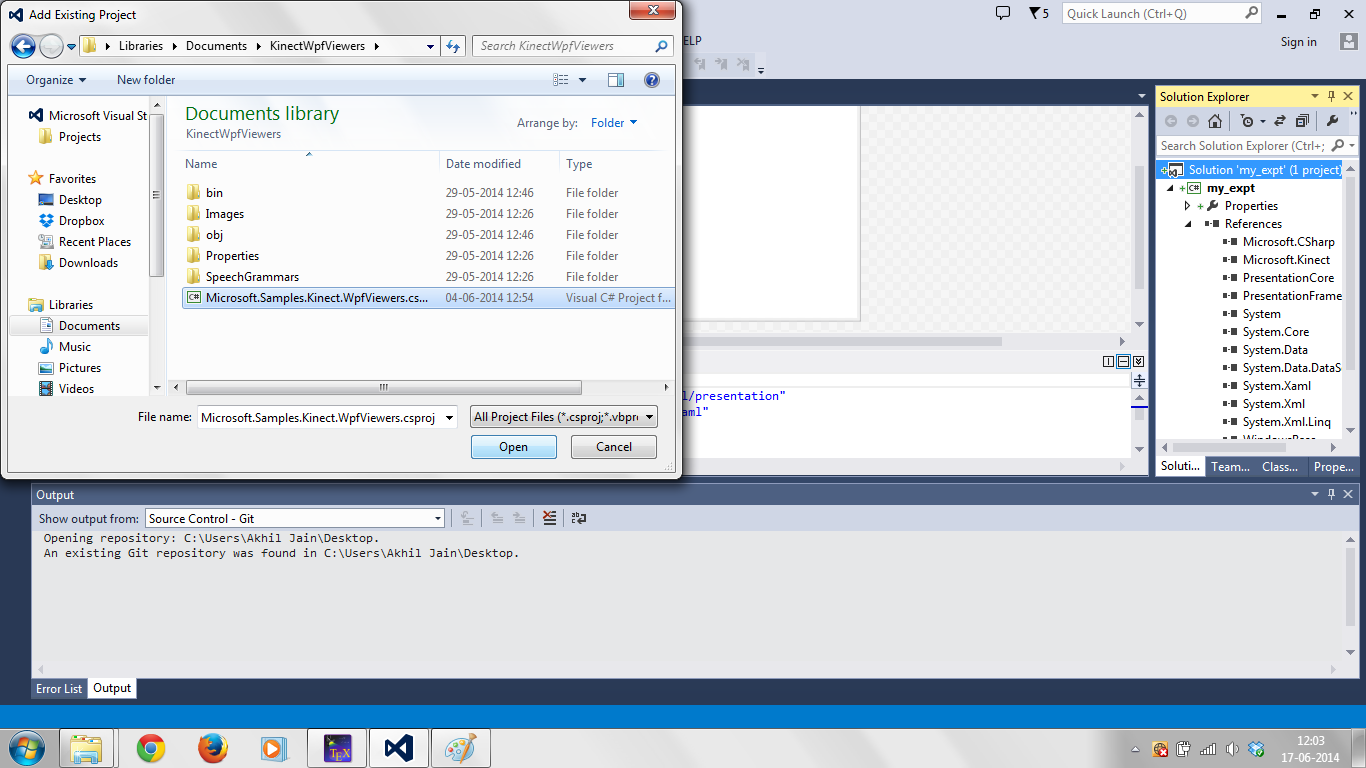
\includegraphics[scale=0.5]{s7}
\end{center}
\caption{Step 7 - Select the project in KinectWpfViewers}
\label{fig:e7}
\end{figure}

\medskip
\begin{figure}
\begin{center}
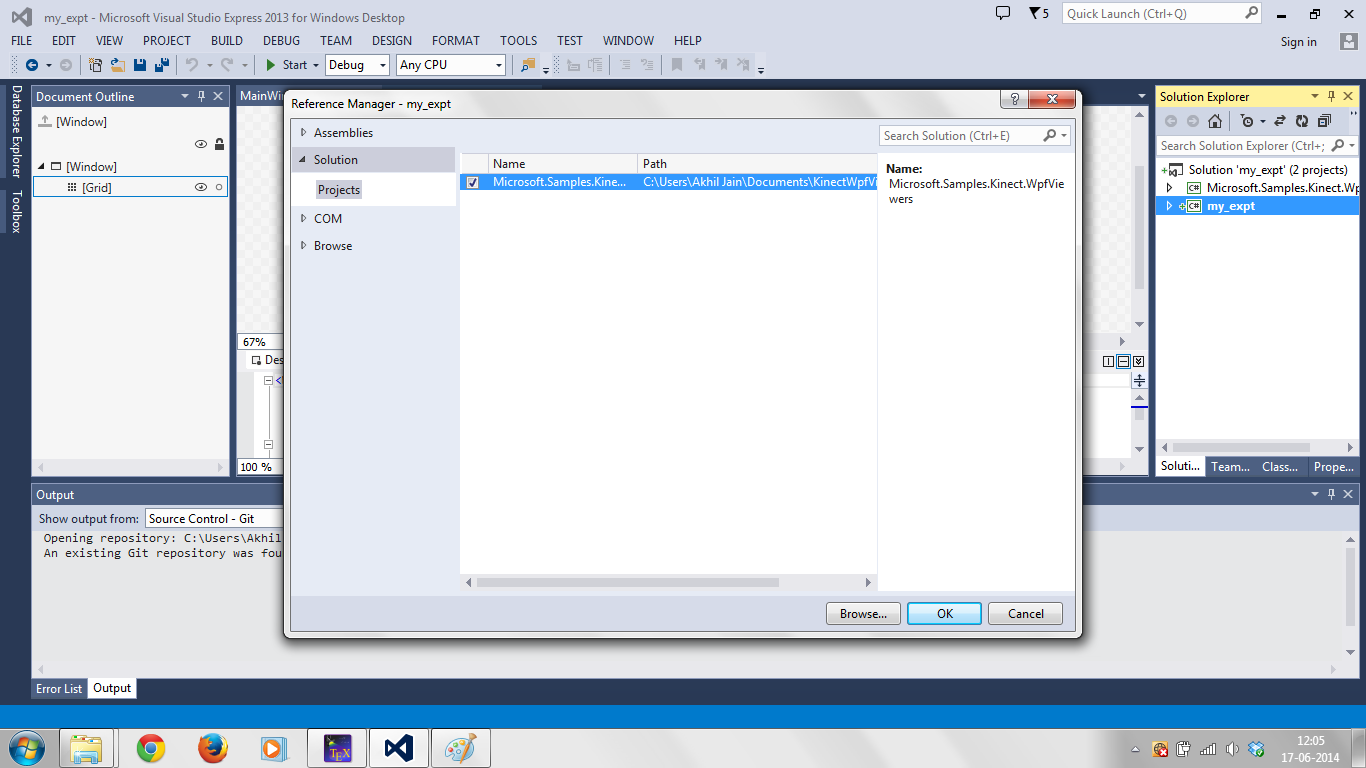
\includegraphics[scale=0.5]{s8}
\end{center}
\caption{Step 8 - Reference the added project}
\label{fig:e8}
\end{figure}

\medskip
\begin{figure}
\begin{center}
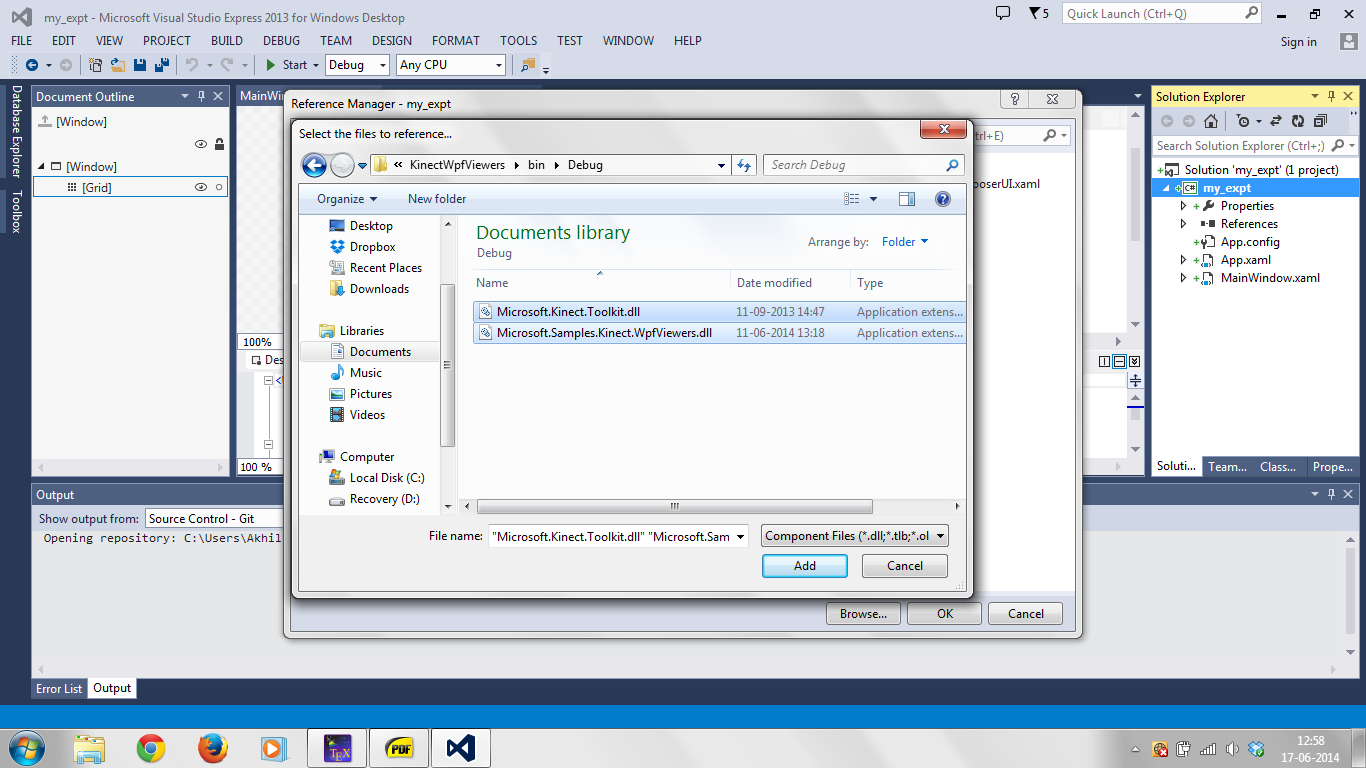
\includegraphics[scale=0.5]{s9}
\end{center}
\caption{Step 9 - Adding final 2 references}
\label{fig:e9}
\end{figure}
\medskip
\begin{figure}
\begin{center}
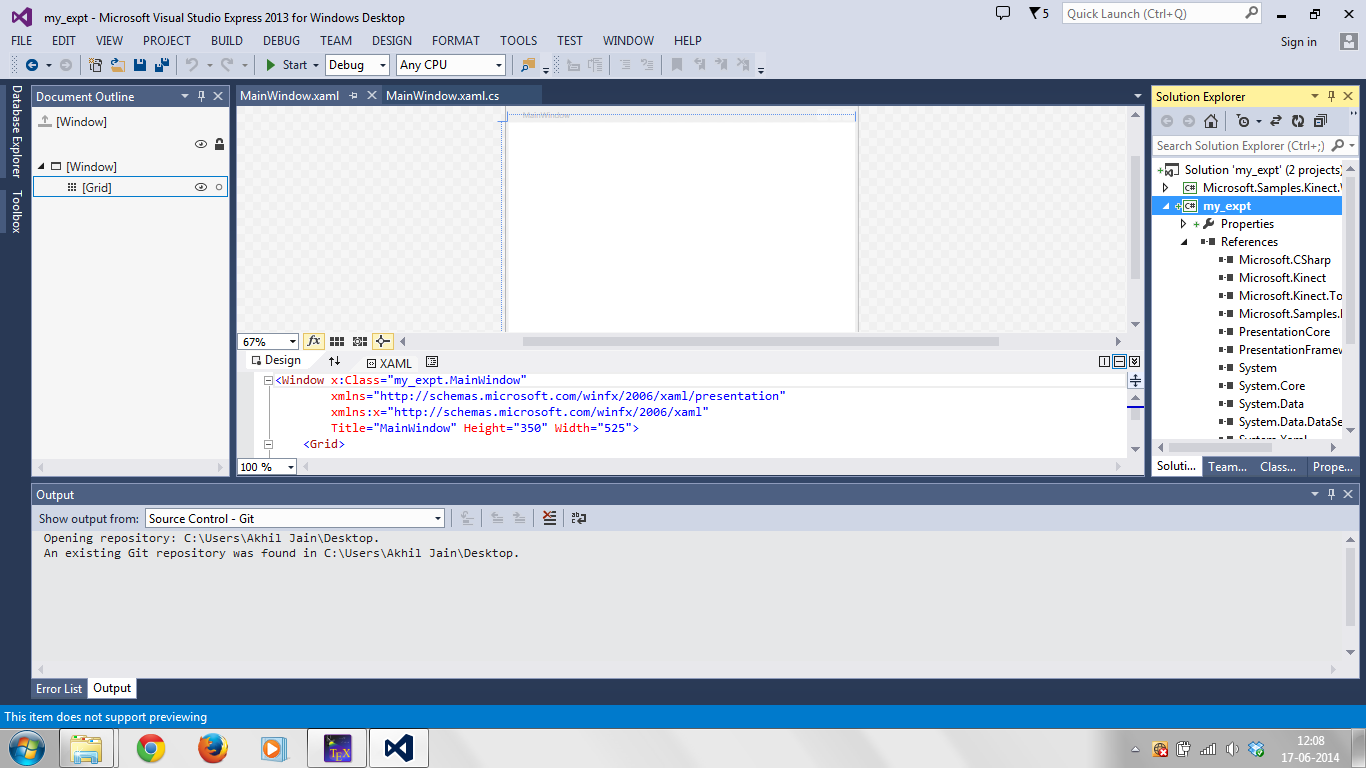
\includegraphics[scale=0.5]{s10}
\end{center}
\caption{Step 10 - Project window post setup}
\label{fig:e10}
\end{figure}
\medskip
\Large{\textbf{Congratulations ! You have successfuly completed the set up on Visual Studio to design codes for working on the Kinect sensor.}}


\end{flushleft}

